\documentclass[a4paper,10 pt]{article} 
\usepackage[french,italian]{babel} 
\usepackage[T1]{fontenc} 
\usepackage[utf8]{inputenc} 
\usepackage{enumitem}
\usepackage{amsmath}
\usepackage{amssymb}
\usepackage{amsthm}                              
\usepackage{graphicx}
\usepackage[normalem]{ulem}
\useunder{\uline}{\ul}{}
\usepackage[a4paper, top=1.27cm, bottom=2cm, left=1.27cm, right=1.27cm]{geometry}
\usepackage{booktabs}
\usepackage{array}
\usepackage {quoting}
\usepackage{subfig}

% Per creare un "blocco" codice
\usepackage{xcolor}
\usepackage{listings}


\colorlet{mygray}{black!30}
\colorlet{mygreen}{green!60!blue}
\colorlet{mymauve}{red!60!blue}

\lstset{
  backgroundcolor=\color{gray!10},  
  basicstyle=\ttfamily,
  columns=fullflexible,
  breakatwhitespace=false,      
  breaklines=true,                
  captionpos=b,                    
  commentstyle=\color{mygreen}, 
  extendedchars=true,              
  frame=single,                   
  keepspaces=true,             
  keywordstyle=\color{blue},      
  language=c++,                 
  numbers=none,                
  numbersep=5pt,                   
  numberstyle=\tiny\color{blue}, 
  rulecolor=\color{mygray},        
  showspaces=false,               
  showtabs=false,                 
  stepnumber=5,                  
  stringstyle=\color{mymauve},    
  tabsize=3,                      
  title=\lstname                
} % fine

\title{\huge{Simulazione diffusione epidemia secondo modello SIR}} 
\author{Anastasi Edoardo \  Lanzi Samuele \ Merola Samuele}
\date{A.A. 2019-2020}

\begin{document}
\maketitle 


\begin{abstract}
 Il nostro programma si sviluppa in due modalità:
 \begin{itemize}
	\item[Modalità 1] Permette di ottenere l'andamento di persone suscettibili, infetti e rimossi in un'epidemia in funzione del tempo. Utilizza come input i valori di $\beta$ e $\gamma$ (valori caratteristici di ogni epidemia) e presenta in output i valori di suscettibili, infetti e rimossi per ogni giorno (vengono simulati 60 giorni, partendo da una situazione di 100 infetti su una popolazione di 1000 unità); i valori in output vengono presentati sia in tabella che in un grafico.
 \item[Modalità 2] Permette di visualizzare in una griglia grafica lo stato di ciascuna unità durante il corso di una epidemia, allo stesso tempo viene stampato il grafico delle curve di suscettibili, infetti e guariti in funzione del tempo nell'epidemia simulata. In input si assegnano le celle da ritenere infette all'origine con click del mouse sulle celle. In output, la situazione dell'epidemia in aggiornamento per ogni giorno fino al termine del contagio.
  \end{itemize}
\end{abstract}



\section{Scelte progettuali e implementative} 
\subsection{Modalità 1}
Il modello SIR è un modello matematico che descrive l'evoluzione di una epidemia. L'andamento di S, I, R è descritto dalle seguenti formule:
$$
S_i = S_{i - 1} - \beta I_{i - 1}S_{i - 1} 
$$
$$
I_i = I_{i - 1} + \beta I_{i - 1}S_{i - 1} - \gamma I_{i - 1}
$$
$$
R_i = R_{i - 1} + \gamma I_{i - 1}
$$
$\beta$ indica la probabilità di contagio ed è compresa tra 0 e 1 e $\gamma$ indica la probabilità di guarigione, anch'essa compresa tra 0 e 1.
\ \\
Il nostro programma utilizza queste formule per calcolare i valori di S, I e R per ogni giorno i-esimo (si veda  \textbf{\textit{sir.cpp}}).
\ \\
%All'avvio del programma, all'utente sarà chiesto di fornire tramite standard input i valori di beta, gamma e infetti iniziali - dati caratteristici della situazione da simulare. 
La durata della simulazione (60 giorni) e il numero totale della popolazione (1000 unità) sono già definiti al compile time. Anche i parametri $\beta$ e $\gamma$ vengono definiti dal programmatore, di default abbiamo assegnato $\beta = 0.0035$ e $\gamma = 0.12$ \footnote{per questi valori abbiamo fatto rifermento a quelli citati dai professori Lamberti, Cifra e Marone del Dipartimento di Matematica dell'Università Sapienza di Roma (https://www1.mat.uniroma1.it/people/pensionati/lamberti/lauree/sir.pdf)} (si veda il \textbf{\textit{main.cpp}})
\\ 
Con questi valori il programma riesce a calcolare i valori di S, I e R di ciascun giorno (si veda  \textbf{\textit{sir.cpp}}) e stamparli come standard output (si veda  \textbf{\textit{print.cpp}}), inoltre in \textbf{\textit{main.cpp}} viene creata una finestra con l'ausilio della libreria SFML, vengono creati tre vettori che contengono le coordinate dei valori di S, I e R in funzione dei giorni trascorsi e i punti vengono stampati in un piano cartesiano su questa finestra.


\subsection{Modalità 2}
Questa modalità prevede di osservare in via grafica l'andamento del contagio in una griglia bidimensionale composta da 256 celle per lato. Ogni cella rappresenta un individuo e può essere di stato S, I o R. Gli individui infetti hanno una certa probabilità di contagiare le celle vicine di stato suscettibile e rimangono infetti per un certo lasso di tempo distribuito uniformemente tra 14 e 20 giorni (si faccia riferimento a \textbf{\textit{person.hpp}}). Definito l'oggetto \verb!Person! e inizializzato come \verb!Susceptible!, in \textbf{\textit{board.hpp}} viene creata la griglia \verb!Board! come vettore di tipo  \verb!Person!. A questo punto il \textbf{\textit{main.cpp}} può, con l'aiuto di SFML, riempire una finestra con una griglia piena di celle. Visivamente (si veda  \textbf{\textit{display.hpp}}) le \verb!Person! di stato \verb!Susceptible! vengono colorate di rosso, le \verb!Person! di stato \verb!Infectious! vengono colorate di verde e quelle di stato \verb!Recovered! di blu.
\ \\
All'avvio del programma l'utente con il mouse dovrà premere su ogni cella che vuole considerare infetta allo stato iniziale e quindi si colorerà di verde. Raggiunto lo stato iniziale desiderato, l'utente darà inizio alla simulazione dei contagi premendo un qualsiasi tasto sulla tastiera. Il \textbf{\textit{main.cpp}} stamperà su terminale il conteggio corrente dello stato delle celle (calcolato in \textbf{\textit{count.cpp}}) aggiornandolo ad ogni ciclo; con questi valori un'altra finestra SFML terrà traccia dell'andamento di S(t), I(t) e R(t) e li graficherà simultaneamente (si vedano le righe 33-116 di \textbf{\textit{main.cpp}}) . Anche la \verb!Board! (e di conseguenza la schermata grafica) si aggiornerà tenendo conto dei contagi. La situazione dei contagi e l'evoluzione delle celle è definita in \textbf{\textit{evolve.cpp}}.

\section{Istruzioni di compilazione e esecuzione}

Per la corretta compilazione del progetto è necessario l'utilizzo di CMake. %e librerie SFML?? <------ !!!
Se non si possiede CMake, è necessario installarlo:
\begin{lstlisting}
	sudo apt-get install cmake
\end{lstlisting}
Anche la libreria grafica SFML è necessaria. Se non la si possiede, si proceda all'installazione così:
\begin{lstlisting}
	sudo apt-get install libsfml-dev
\end{lstlisting}
Dopo aver installato CMake, si può passare alla compilazione:
\begin{lstlisting}
	cd SIRmodel
	cd option1 (cd option2)
	mkdir build
	cd build
	cmake -DCMAKE_BUILD_TYPE=Debug ..
	cmake --build . --target all
	make VERBOSE=1 
\end{lstlisting}
Ora il progetto è compilato, si può procedere con i test tramite il comando
\begin{lstlisting}
	ctest
\end{lstlisting}
oppure con l'esecuzione del programma tramite il comando
\begin{lstlisting}
	./sir-sfml
\end{lstlisting}
\section{Risultati output e interpretazione}
\subsection{Modalità 1}
Eseguendo la prima modalità del programma, verranno mostrati in output del terminale tramite uno  \verb! std::cout ! i valori di S, I e R per ogni giorno di simulazione [Figura 1 (a)]; inoltre, grazie alla libreria SFML, verrà aperto un grafico che rappresenta tali valori in funzione dei giorni trascorsi. Si vedranno quindi dei punti rossi che rappresentano il numero di persone suscettibili per giorno, dei punti blu che rappresentano i non suscettibili per giorno e dei punti verdi che rappresentano quanti sono infetti in quel giorno [Figura 1 (b)]. Si può notare che il risultato è coerente con il modello SIR atteso (si veda Scelte progettuali e implementative).


\begin{figure}
\centering
\subfloat[][\emph{output tramite finestra grafica SFML}]
{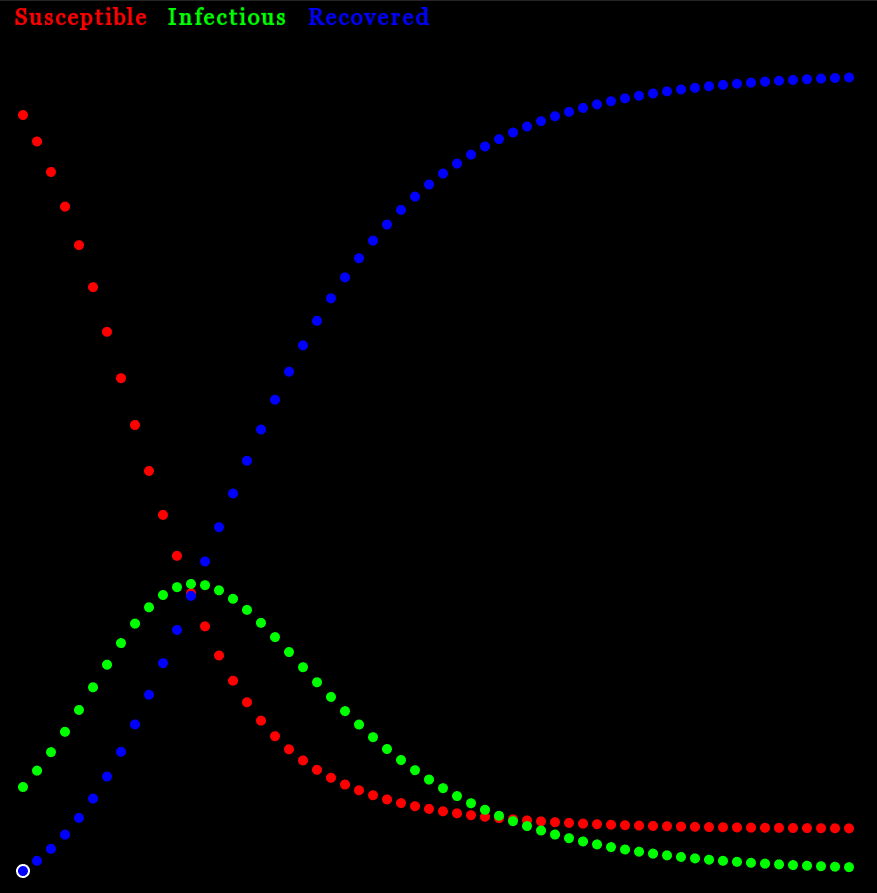
\includegraphics[width=.60\textwidth]{Figura_1.png}} \quad \subfloat[][\emph{standard output da terminale}]
{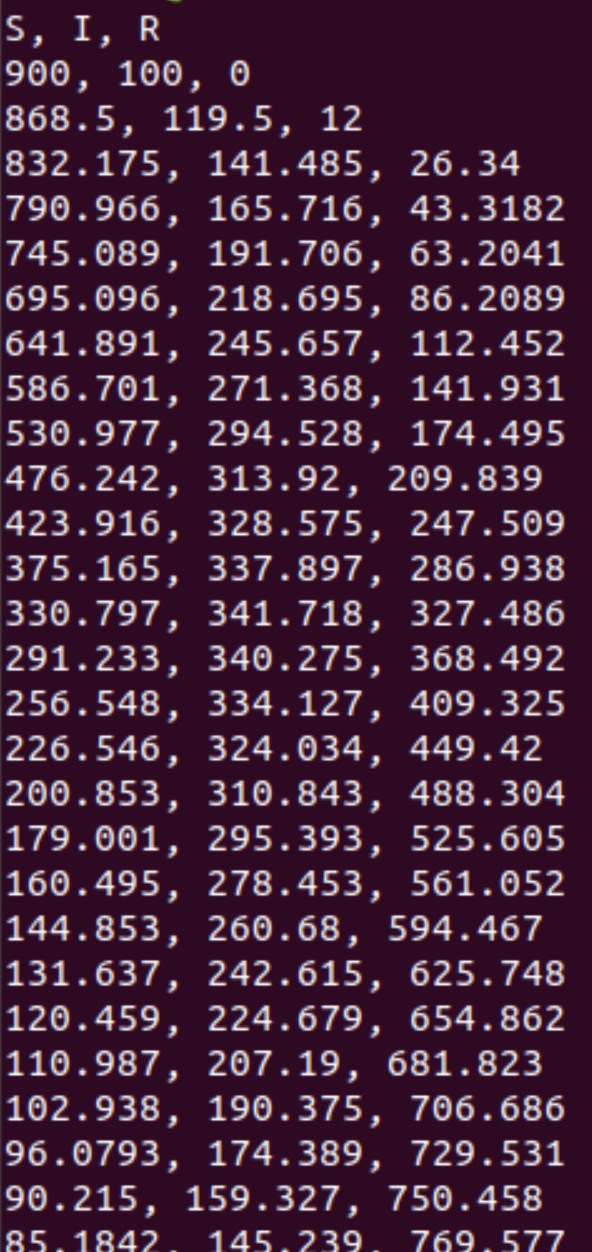
\includegraphics[width=.25\textwidth]{Figura_2.png}} \\
\caption{}
\label{fig:subfig}
\end{figure}


\subsection{Modalità 2}
Eseguendo la seconda modalità del programma, dopo aver scelto le celle infette allo stato iniziale (come descritto in Scelte progettuali e implementative), si darà il via alla simulazione premendo un tasto della tastiera. La griglia con le celle [Figura 2(a)] si aggiorna ogni 30ms che rappresenta un giorno, le persone infette rimarranno tali per un numero di giorni distribuito uniformemente tra 14 e 20. Ad ogni ciclo la griglia mostrerà lo stato i-esimo di ciascuna cella facendone variare il colore. Contestualmente, nell'altra finestra [Figura 2 (b)] vengono graficati i valori di S(t) I(t) e R(t) conteggiando i valori reali dell'attuale simulazione. Al termine della simulazione si potranno osservare quante celle sono state colpite dall'epidemia e quante sono ancora suscettibili, mentre nel grafico si potrà apprezzare l'andamento in funzione dei giorni trascorsi.


Il programmatore, prima della compilazione, stabilisce un valore di contagiosità \verb!constexpr int probabilityToInfect! (tra 0 e 100) in \textbf{\textit{person.hpp, line 9}}. Utilizzando valori differenti si vede come può evolvere l'epidemia: inserendo un'alta probabilità di contagio l'epidemia procederà rapidamente e in pochi giorni gran parte della popolazione risulterà infetta, al contrario inserendo una probabilità molto bassa si vede che l'epidemia rallenta fino a cessare prima di infettare molte celle.

\begin{figure}
\centering
\subfloat[][\emph{griglia 256x256 rappresentante la situazione di ogni individuo}]
{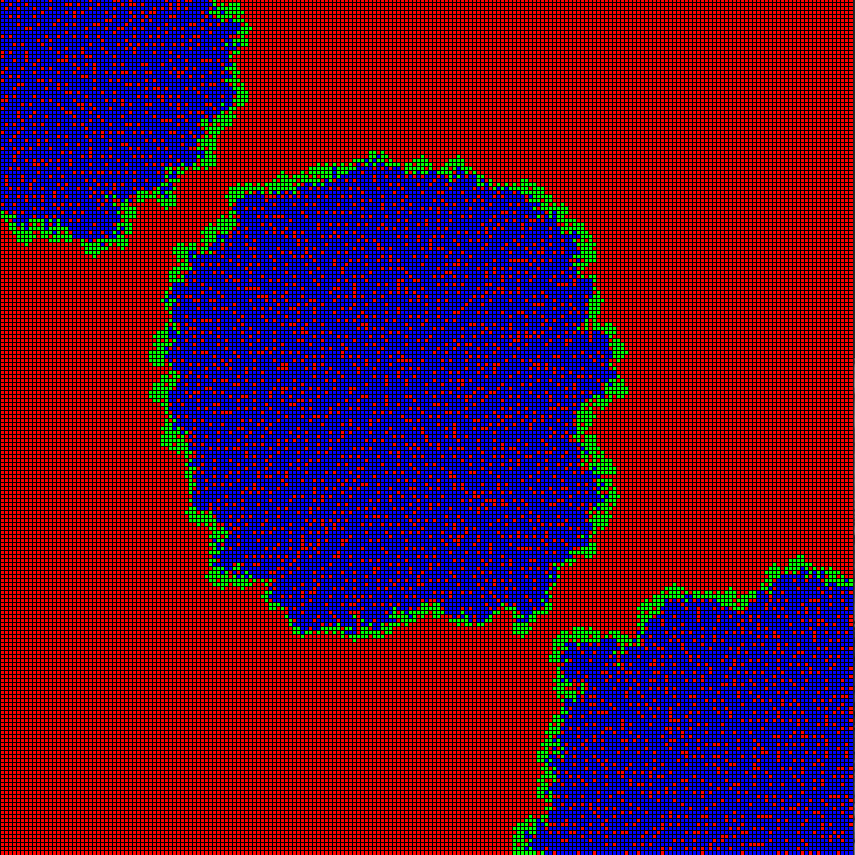
\includegraphics[width=.45\textwidth]{Figura_3.png}} \quad \subfloat[][\emph{grafico della situazione di contagio secondo il modello attuale}]
{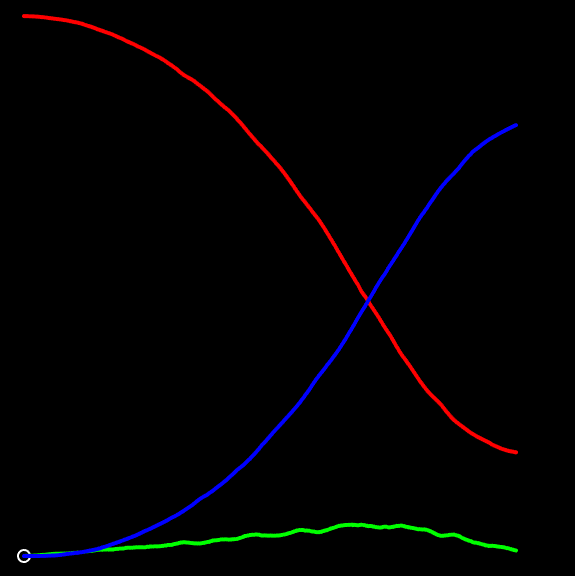
\includegraphics[width=.45\textwidth]{Figura_4.png}} \\
\caption{}
\label{fig:subfig}
\end{figure}

\section{Test e condizioni per la corretta esecuzione}
....
\ \\
....
\ \\
...includi in questa sezione i test, gli assert e try 
\ \\
.....
\ \\
...
\ \\
....
\end{document}
